\documentclass[Dissertation.tex]{subfiles}
\begin{document}
\chapter{Dataset and Problem Statement}
This chapter investigates the structure and content of the Brexit Blog Corpus, beginning with an informal description of the data followed by numerical and visual analysis.
\section{Dataset Description} \label{Data}

The dataset comprises 1,682 utterances  labelled for speaker stance according to a framework of ten notional categories of speaker stance \cite{simakiAnnotatingSpeakerStance2017}. The utterances are extracted from political blog posts related to the United Kingdom 2016 EU membership referendum \cite{simakiAnnotatingSpeakerStance2017}. The manual annotation procedure in \cite{simakiAnnotatingSpeakerStance2017} is described as follows: two annotators from linguistics backgrounds were each asked to annotate each utterance with up to five of the ten notional stance categories. The annotators were also asked to repeat the process, in order that there be two sets of annotations from each annotator, allowing inter-annotator and intra-annotator agreement scores to be calculated. Where there was significant divergence between annotations, utterances were discussed by the annotators and final annotation was agreed upon. 

Below in Table \ref{tab:stanceExamples} are brief definitions of each stance category together with two sentences demonstrating each category. Each example contains stance characterising elements of varying lengths. For example, {\small\scshape Necessity} can be expressed with individual stance markers such as \textit{must}, but also with longer phrases such as \textit{there is no other way}. It is important to note that the categories are not mutually exclusive, and utterances in the dataset can have multiple labels. Table \ref{tab:dataExtracts} shows several extracts from the data set, including utterances with multiple labels. Intuitively it can be seen that some stance markers relate to more than one category. For example, a sentence containing the stance marker \textit{I think} could be categorised as {\small \scshape Hypotheticality}, {\small \scshape Uncertainty}, or both. There are also natural relationships between categories. While hypothetical constructions inherently contain a prediction, Simaki et al. instructed annotators to label such instances as {\small \scshape Hypotheticality} only In this Chapterrather than {\small \scshape Hypotheticality} and {\small \scshape Prediction} \cite{simakiAnnotatingSpeakerStance2017}.

{\renewcommand{\arraystretch}{2.5}
	\centering
	\begin{table}[]
		
		\begin{tabularx}{\textwidth}{>{\raggedright}p{3cm} >{\raggedright}p{5.5cm} X}
			\toprule
			Stance Category        & Description                                            & Examples                                                                                                                                      \\ \midrule
			\small\scshape Agreement/ Disagreement &Utterance aligns with or against an opinion &\itshape That is the wrong approach. \par I believe this a good idea.\\
			\small\scshape Certainty              &Utterance shows conviction or confidence in statement& \itshape It is absolutely clear. \par Without a doubt this is possible.                                          \\
			\small\scshape Contrariety            & Utterance shows compromise or comparison               & \itshape Some think this is good, but others disagree.\par We have come far,  but there is still much to be done\\ 
			\small\scshape Hypotheticality        & Utterance describes consequences of a premise          &\itshape If that happened, it would be a disaster.\par I would be happy if he won.                              \\
			\small\scshape Necessity              & Utterance expresses an obligation or a request         & \itshape You must do it.\par I have to be there.                                                                \\
			\small\scshape Prediction             & Utterance shows speculation                            &\itshape The match should be an easy win.\par I think the journey will go by quickly.                           \\
			\small\scshape Source of Knowledge    & Utterance refers to the origin of opinion or statement & \itshape James told me he is moving house.\par The film was rated highly in the newspaper.                      \\
			\small\scshape Tact/Rudeness          & Utterance is either  polite or abrasive           & \itshape I would be grateful if you do this.\par I couldn’t give a damn how you feel.                           \\
			\small\scshape Uncertainty            & Utterance admits doubt                                 & \itshape To be honest I am not sure.\par I can’t guarantee I can make it.                                       \\ \bottomrule
		\end{tabularx}
		\caption{Stance categories, descriptions and examples}
		\label{tab:stanceExamples}
\end{table}}

{\renewcommand{\arraystretch}{1.5}
	\centering
\begin{table}
	\begin{tabularx}{\textwidth}{>{\raggedright}X >{\raggedright \arraybackslash}p{5cm}}
		\toprule
		Utterance 											& Stance Categories \\ \midrule
		\itshape It might help us to solve some of the intractable problems in the world and start to move forward. &\small\scshape Uncertainty \\
		\itshape Under the Fixed-term Parliaments Act 2011, elections now take place every five years, unless an early election is triggered. &\small\scshape  Hypotheticality, Source of Knowledge \\
		\itshape Of course, this is far from the dominant narrative we hear in the media. & \small\scshape Agreement/Disagreement \\
		\itshape They’ll trade alright, but any post brexit EU trade agreement will have a stiff price attached as Norway will testify. &\small\scshape  Contrariety, Prediction\\
		\itshape Yes, we want worker protection, but we don’t need to go over the top as the EU does. & \small\scshape Necessity, Contrariety, Volition\\
		\itshape I’m glad that you stated your position so clearly in your last post. &\small\scshape  Tact/Rudeness
		 \\\bottomrule
		
	\end{tabularx}
\caption{Dataset Extracts
\label{tab:dataExtracts}}
\end{table}}
\section{Problem Statment}

\section{Exploratory Data Analysis}
Before Dev


\begin{figure}
	\centering
	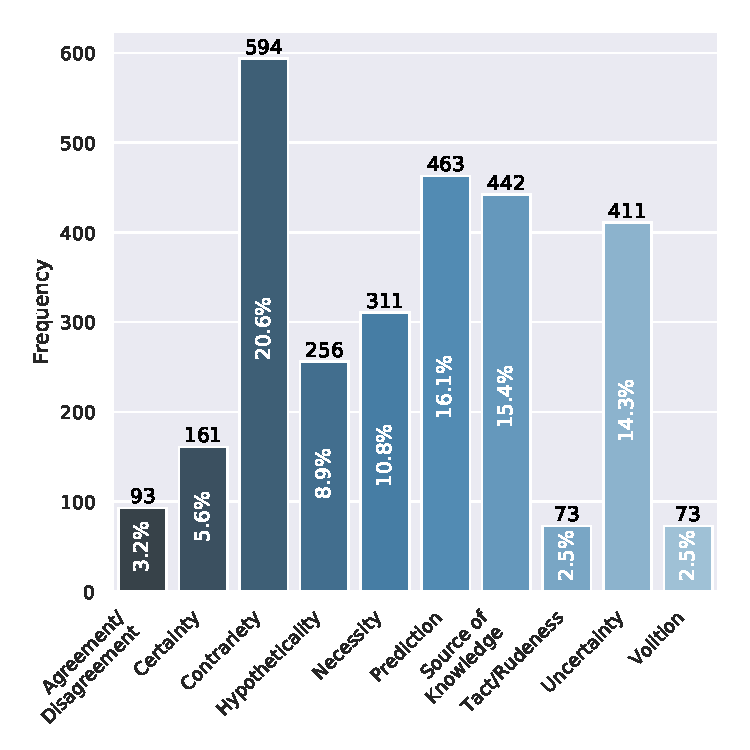
\includegraphics[width=5in]{label_counts.pdf}
	\caption{Bar chart of label counts}
\end{figure}

\begin{figure}
	\centering
	\hspace*{1em}
	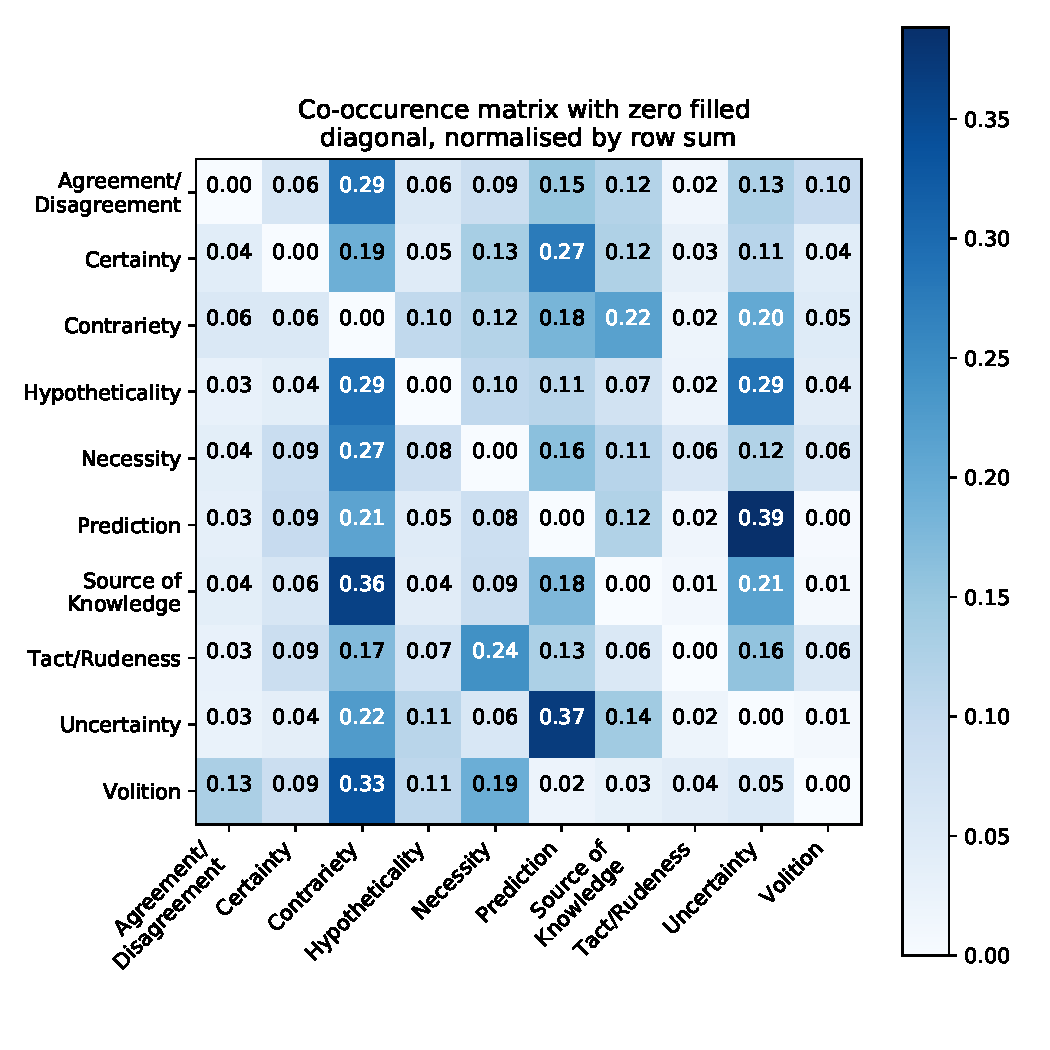
\includegraphics[width=5in]{label_confusion_matrix.pdf}
	\caption{Label co-occurence matrix heatmap}
	\label{fig:labCoOc}
\end{figure}




\end{document}